\chapter{On Chip SRAM}

\begin{figure}[htbp]
    \centering
    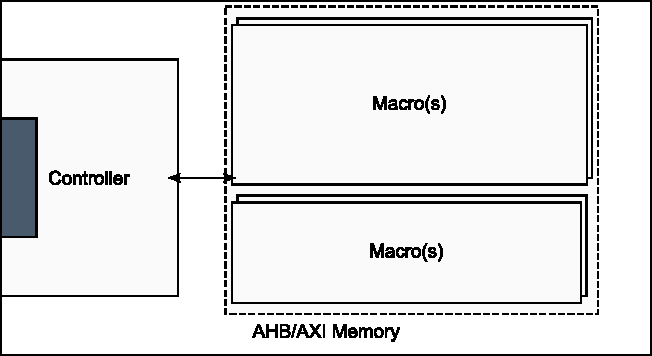
\includegraphics[width=0.55\textwidth]{figures/sram_module_blk.pdf}
    \caption{AXI/AHB SRAM module general block view.}
    \label{fig:sram-module-blk}
\end{figure}

\section{Overview} 
SRAM macros usually expose a simple interface. Such an interface is seldom compatible with the port interfaces exposed by Network on Chip (NoC) or Network Interconnects (NIC). These systems employ elaborate on-chip interconnect standards like AHB/AXI\footnote{None of the AMBA Bus protocols will be discussed in detailed here. Please refer to the \textbf{official} documentation(s) available online.} as they need to handle multiple transactions from multiple devices concurrently. Such protocols include transaction-related metadata signals which enable this capability. We require a controller frontend that will consume these highly informative AHB/AXI transactions and translate it into low-level SRAM interface access(es). We first provide a brief overview of the common controller logic for each of the protocol and then conclude with a description of the generator utility provided. Figure~\ref{fig:sram-module-blk} shows the common block view of the SRAM module. The macros are instantiated independently of the controller via rule checking if using the optional configurator. Named \texttt{gen\_lib\_sram\_*}, the user is expected to replace these prior to synthesis and/or pd with actual models from the foundry.  

\section{AHB Controller}

The AHB family of macros uses \texttt{ahb2sram}, a 32-bit\footnote{At the time of writing this, the controller only supports and is tested for 32-bit word size.} AHB-Lite subordinate for a single-port synchronous SRAM. This controller module is parameterized with the geometry of the module the user expects. This can be different from the configuration of SRAM macros available to the user. The optional generator tool, discussed later, is capable to combining available macros to match the user's specific requirements. 

\underline{Controller Parameters}:
\begin{enumerate}
    \item \texttt{LINE\_W}: required SRAM line width in bits
    \item \texttt{LINE\_AW}: use to define the depth (\(2^{\texttt{LINE\_AW}}\)) of the SRAM in bits
    \item \texttt{WORDS}: number of 32-bit words. The current controller is only capable of supporting 32-bit words. Hence, this parameter should always equal \(\texttt{LINE\_W} / 32\).
\end{enumerate}


\subsection{AHB-Lite Primer}
An AHB-Lite transfer is split across two pipelined phases - address phase (aphase) and data phase (dphase). In the aphase the manager drives \texttt{HADDR}, \texttt{HTRANS}, \texttt{HWRITE}, and \texttt{HSIZE}, qualified by \texttt{HSEL} and the shared \texttt{HREADY}. In the subsequent dphase, write data (\texttt{HWDATA}) or read data (\texttt{HRDATA}) is exchanged, with the subordinate controlling the bus through its registered \texttt{HREADYOUT} and reporting status on \texttt{HRESP}. \texttt{HTRANS[1]} distinguishes an active (\texttt{NONSEQ}/\texttt{SEQ}) beat from \texttt{IDLE}/\texttt{BUSY}. Our implementation does not support burst-type transfers. This is in align with the behavior of the PicoRV32 core's native memory interface. 

\subsection{Phase Sequencing and Timing}
The least significant bits of the address are word alignment bits and will be always zero for word size greater than 8 b. The next significant bit(s) are used for word select for wide SRAM lines.  
An active address beat is registered on \(\texttt{aphase} = \texttt{HSEL}\ \&\ \texttt{HREADY}\ \&\ \texttt{HTRANS[1]}\). A read drives the SRAM in the same cycle and its data is returned in the data phase; a write is held one cycle so that its data phase supplies \texttt{HWDATA}. Consequently a read incurs no wait state and a write incurs exactly one. 

The chip enable, global write enable, and address to the macro are
\[
\texttt{CEN} = \sim(\texttt{read\_en} \mid \texttt{write\_en\_reg}), \quad
\texttt{GWEN} = \texttt{read\_en}, \quad
\texttt{A} = \texttt{read\_en}\ ?\ \texttt{line\_addr\_nxt} : \texttt{line\_addr\_reg},
\]
so a read presents the incoming address immediately while a write replays the registered one.

\subsection{Byte Lanes and Write Enables}
From \texttt{HSIZE} and the lower address bits the controller derives a one-hot-per-byte lane mask (byte, half-word, or full word), registers it into the data phase, and expands it into the macro's active-low, bitwise write enable. When a line is wider and can accomodate several bus-words (\(\texttt{WORDS} > 1\)) the addressed 32-bit word is selected within the line for both the write mask and the read data; otherwise the line is the word. On a read the registered byte lanes gate \texttt{HRDATA}; \texttt{HRESP} is tied to \texttt{OKAY}.

\section{AXI Controller} 

\begin{figure}[htbp]
    \centering
    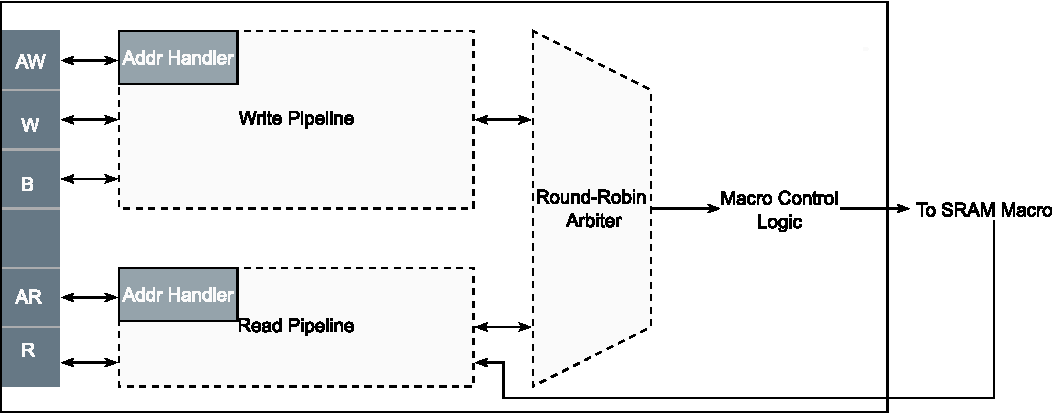
\includegraphics[width=0.75\textwidth]{figures/axi2sram_blk.pdf}
    \caption{\texttt{axi2sram} controller detailed block view.}
    \label{fig:axi2sram-blk}
\end{figure}

Similar to the AHB controller, there is an AXI controller (\texttt{axi2sram}) that converts AXI transactions to SRAM control logic. However, AXI is a more complex (and thereby capable) protocol compared to AHB. Figure~\autoref{fig:axi2sram-blk} provides an overview of the architecture of this controller. Note that the dotted lines are only meant to represent sections of the logic and are not implemented as independent sub-modules. Only the address handler module that is shared by the both pipelines is implemented separately as a module.  

\subsection{AXI Addressing Primer} 

Most of the understanding about AXI addressing has to do with Burst transactions. Burst transactions involve multiple transfers. In these, the manager is expected to provide only a start address and the subordinate is expected to handle the rest of the transfers based on that address and some control signals.  

There are two key control signals:
\begin{enumerate}
    \item \texttt{AxSIZE}: This signal carries information about the number of bytes of information accessed in each transfer (also called a beat) within a Burst transaction. Specifically, 
    \begin{equation*}
        \text{Number of bytes} = 2^{\texttt{AxSIZE}}.
    \end{equation*}
    The width of this signal and the value it can assume is constrained by the data width. AXI doest not permit packet sizes greater than size of the Data bus. The width can be calculated as follows:
    \[
    \text{Width} = \$\texttt{clog2}\left(\frac{\texttt{DW}}{8}\right).
    \]
    (\$\texttt{clog2} rounds up; for a power-of-two \texttt{DW}/8 it is exact.)
    \item \texttt{AxLEN [7:0]}: This indicates the number of transfers to be completed within a single Burst transaction. Specifically,
    \[
    \text{Number of transfers} = 1 + \texttt{AxLEN}
    \] 
\end{enumerate}
Here \texttt{Ax} stands for \texttt{AW} or \texttt{AR}.

There are three types of Burst transactions possible: \begin{itemize}
    \item FIXED: In a Burst type of FIXED type, same address is used repeatedly. An example application provided in the AXI specification is for emptying a FIFO. Generally, used very little.   
    \item INCR: INCR Burst transactions are more common and align with the intuitive picture of a burst transfer. It sequential increments the address until specified.
    \item WRAP: A WRAP Burst transaction is similar to INCR, except it wraps around at a specific boundary depending on transaction attributes. 
\end{itemize}

AXI ``Regular'' transactions impose certain restrictions on the attributes of the trasactions. See section A3.1.8 of AMBA IHI0022 document.  Of those, our address generation submodule (\texttt{axi\_addr\_handler}) assumes the following:
\begin{enumerate}
    \item Number of transfers: INCR bursts of \(1\)--\(256\) beats; WRAP bursts of \(\{2, 4, 8, 16\}\) beats.
    \item Size is the same as the data channnel if Length is greater than 1.
    \item Address is aligned to the transaction container for INCR transactions.
    \item Address is aligned to Size for WRAP transactions.  
    \item Transactions are not permitted to cross a 4KB boundary (section A3.1.3, AMBA IHI0022)
\end{enumerate}

\subsection{Implementation} 

The AXI memory module consists of the following components: Main controller logic for handling AXI transactions, a submodule for handling burst addressing, and the native interfaced, SRAM macro. Here only discuss the controller. The SRAM macro exposes a read port (Q), write port (D), clock (CLK), chip enable port (CEN), global write enable (GWEN), local write enable (WEN), address port (A), and additional signals\footnote{These are ignored for simulation purposes.}, STOV, EMA, EMAS, EMAW.

\begin{enumerate}
    \item Handling the addressing:
    
    The module \texttt{axi\_addr\_handler} is responsible for handling the addressing during Burst transactions. Given a start address, type of burst transfer, size of each transfer, and length of transaction, it generates addresses for each beat of the transaction. It is implemented as a two state FSM: IDLE and ACTIVE. It accepts new start address (called descriptor in the source code) whenever it is in IDLE state. This is indicated to the external environment by asserting the \texttt{start\_addr\_ready} signal. Once the external module asserts \texttt{start\_addr\_valid} signal, this module samples all the input signals, registers them, and enters ACTIVE state. Once in ACTIVE, it uses a count-down timer to track each beat. On the last count, the \texttt{is\_last\_addr} flag is asserted and the FSM moves into IDLE state. The module uses the \texttt{next\_addr\_ready/valid} handshake to move to the next address in the Burst transaction. 

    The next address for Burst transactions is calculated as follows:
    \begin{align}
        \texttt{next\_addr} = \begin{cases}
            \texttt{curr\_addr} & \text{if } \texttt{AxBURST = `FIXED}\\
            \texttt{curr\_addr} + 2^{\texttt{AxSIZE}} & \text{if } \texttt{AxBURST = `INCR} \text{ or within wrap boundary when } \texttt{AxBURST = `WRAP}  \\
            \texttt{wrap\_base} & \text{if } \texttt{AxBURST = `WRAP} \text{ and crossing wrap boundary.}
        \end{cases}
    \end{align}
    Here, \texttt{wrap\_base} is the aligned base of the wrap region. Refer to the AXI specification for how this might be calculated\footnote{WRAP Burst is intended for cache implementations, where, to minimize stall penalty, the first word is delivered immediately and the the rest of the cache line is then fetched sequencially (wrapping).}. This module assumes that the start address is aligned to Size and one increment indicates a word-size (element) increment of \(2^{\texttt{AxSIZE}}\) bytes, i.e., the byte address will be incremented by 4 if Size = 4 bytes. Cache accesses is the main motivation of WRAP Bursts.

    AXI4 limits the length of WRAP transactions to 2/4/8/16. This provides a neat little trick used to calculate the next address in a Wrap transaction without using the modulo operator\footnote{Credits for this trick: \href{https://zipcpu.com/blog/2019/04/27/axi-addr.html}{https://zipcpu.com/blog/2019/04/27/axi-addr.html}.}\footnote{My instinct is that they limit the length for Wrap Bursts for this very reason. Or it may just be that 16 is sufficient for most applications.}. For these Lengths, the value of \texttt{AxLEN} is 0001, 0011, 0111, 1111, respectively. Notice that once the address has been adjusted for word alignment (i.e., those least significant zeros are shifted out), then only the bit positions where there is a 1 in value of \texttt{AxLEN} should be changed in the address (when \texttt{AxLEN}) is aligned with least significant end of the address. Rest of the address should carry over from the before. This trick is realized with the following equation:
    \begin{align}
        \texttt{next\_addr\_wrap} = (\texttt{wrap\_mask}\ \&\ \texttt{next\_addr\_incr}) \mid (\sim \texttt{wrap\_mask}\ \&\ \texttt{curr\_addr}).
    \end{align}
    In the above expression, most of the terms should be self-explanatory, except perhaps \texttt{wrap\_mask}. This term is simply the \texttt{AxLEN} signal shifted to account for the word alignment and padded for address size. Bitwise complement of wrap mask has 1 in bit positions that should not change and be carried over from current address. 

    \item Main Controller Logic 
    
    The main controller is implemented to try and mimic the behavior of \texttt{IntMemAxi} IP from ARM, which is a licensed IP that cannot be open-sourced. However, its functionality is described and can be found \href{https://support.arm.com/documentation/dto0009/a/about-the-internal-memory-interface?lang=en}{here}. However, we cannot guarantee the identical behavior as our development was independent of this IP. 

    This module is designed for controlling a single-port SRAM module. The reads and write paths are implemented independently and arbitrated in a round-robin fashion with reads being the default mode. 
    \underline{Controller Parameters}
    \begin{enumerate}
        \item \texttt{DW}: Word Size (only supports 32/64-bit)
        \item \texttt{IDW}: AXI ID signals width
        \item \texttt{LINE\_W}: required SRAM line width
        \item \texttt{LINE\_AW}: use to define the depth of SRAM (in bits)
        \item \texttt{WORDS}: Number of words per SRAM line 
        \item \texttt{READ\_WAIT}: (0/1) Number of wait stages for reads. 
    \end{enumerate}
    
    This controller can support multiple words per SRAM line. Further, the reads can have an optional wait stage that allows pipelining. Note that like the AHB controller, the WORDS parameter should be sensible and will depend on the word size and the line width.

    The write path is relatively straightforward. Whenever a new write request arrives, the address handler is used to unravel and stream the addresses in the burst sequence. Once available and the previous transaction is completed, a new request write request is raised. 
    
    The read path is slightly more complicated by the optional wait state. Whenever a new read request is granted by the arbiter, the read path becomes busy and the count down timer is topped up. Once the count down is complete, the read value appears on the read port of the macro and is subsequently transferred to \texttt{RDATA} bus when it is available. 

    Both, read and write, paths are pipelined to improve performance. Further, similar to AHB controller, rest of the logic is used to generate the line-wide masks by extending the Strobe signals and word select bits. 
\end{enumerate}

\section{Libremc} 

\begin{docnote}
Terminology: We use ``module'' refers to the entity that actually connects to a bus or a network on chip. The user specifies the module geometry. ``Macro'' is used to refer to the actual SRAM provided by the foundry/memory compilers. Such macros have a primitive interface and might have limited configurations. 
\end{docnote}

We provide a support utility called Libremc (short for Libre macro compiler) that enables the SoC configurator to easily build SRAM modules for connecting to either Pico subsystem or the NoC Subsystem. Consequently, it can configure the \begin{enumerate}
    \item Frontend protocol: Either AXI or AHB.
    \item Width (W): width of the SRAM module.
    \item Depth (D): depth of the SRAM module. 
\end{enumerate}
The word size is fixed to 32 bits for AHB slave memories and to 64 bits for AXI ones\footnote{This is because the bus specifications are a part of the architecture which is common to the platform.}. Further, the address bus width is fixed to 32 bits. 

However, often when synthesizing memory modules, one might not have access to the SRAM compilers or the available compilers might have limited capability and only a few macro configurations are accessible. Libremc allows the user to specify the available macro configurations in a \texttt{.conf} file as follows:

\begin{doccode}
\## Depth        Width   DepthStride  WidthStride  Mask-Granularity
16384          32      0            0            8
16384          64      0            0            8
4096           64      0            0            8
8192           64      0            0            8
512-8192       32      512          0            8
\end{doccode}
The values can be specified explicitly or as (low - high) ranges.  

The tool uses this information to find the ``optimal'' combination to meet the user specified module requirements. To keep things simple, we solve a simple grid problem. For each available macro \(m_i = (w_i, d_i)\) configuration, the following cost function \(f_i\) is evaluated:
\begin{align}
    f_i = c_i \times r_i \times a_i,
\end{align}
where, \(c_i = \mathrm{ceil}(W / w_i)\), \(r_i = \mathrm{ceil}(D / d_i)\), and \(a_i\) is the area of macro. When unavailable, the area of the macro can be estimated as the product of a macro's width \(w_i\) and depth 
\(d_i\)\footnote{This does not capture the wiring overhead and may not correlate well with the actual area. We are working to include this wiring overhead to improve this tool.}. 

The tool selects the configuration as follows:
\begin{enumerate}
    \item Configuration with the lowest value of cost function.
    \item Any ties are broken by choosing the configuration with lowest number of instances (\(r_i \times c_i\)).
    \item Remaining ties are broken by choosing the configuration using the smallest macro.
\end{enumerate}

Once a configuration is found, the tool then automatically generates the module RTL along with a configuration file specifying the chosen macro and grid parameters. In this generated SRAM module it instantiates the requested controller and the grid of macros. In addition, it outputs the word select logic.

\subsection{Usage} 

\begin{enumerate}
    \item Generate a memory module: \begin{verbatim}
        $ make gen PROTO=<ahb|axi> SIZE=<lines>x<width> [MACROLIST=<file>.conf]
    \end{verbatim}
    \item Elaborate and test a generated module: \begin{verbatim}
        $ make test-one PROTO=<ahb|axi> SIZE=<lines>x<width> [EXTRA_AW=n]      
    \end{verbatim} 
    \item Generate and test a memory module in one step: \begin{verbatim}
        $ make test PROTO=<ahb|axi> SIZE=<lines>x<width> [MACROLIST=<file>] [EXTRA_AW=n]
    \end{verbatim}
    \item Clean up generated files: \begin{verbatim}
        $ make clean
    \end{verbatim} 
\end{enumerate}

\section{Summary}

While the AHB controller logic was mostly inherited from Base-SoC (ARM), the AXI controller was developed in-house. AXI's Internal memory interface\footnote{\href{https://support.arm.com/documentation/dto0009/a/about-the-internal-memory-interface?lang=en}{https://support.arm.com/documentation/dto0009/a/about-the-internal-memory-interface?lang=en}} behavior combined with SRAM Macro interface were used as a reference. We improved upon the IntMemAxi module\footnote{We abide by the licensing terms by not using the source code for development of our own version. The functionality has been independently replicated.} by directly supporting AXI4 (it supported AXI3) and directly generating the SRAM interface. 

\begin{docwarning}
Testing the Libremc utility is a non-trivial exercise and in fact a tedious one. Hence, we would appreciate any feedback on the tool, bug finds/fixes in the source code, and inaccuracies in this document.
\end{docwarning}